\chapter{Protección de transformadores de distribución}
\section{Protecciones de transformadores}
\subsection{Protección contra sobrecargas}
\begin{itemize}
	\item Interruptores accionados por relés de sobreintensidad
	\item Dispositivos térmicos que detecten la temperatura del devanado o del medio
	refrigerante.	Excepto en el en caso de que dispongan de un sistema de monitorización
	de la evolución de las cargas en tiempo real
\end{itemize}
\subsection{Protección contra cortocircuitos}
\begin{itemize}
	\item Todos los transformadores estarán protegidos contra cortocircuitos
	\item Si el cortocircuito es externo se protege en el lado de salida
	\item Si el cortocircuito es interno protección en el circuito de alimentación
	\item \textbf{Para S$>$1000kVA} protección con interruptor automático
\end{itemize}
\subsection{Protecciones contra sobretensiones}
\begin{itemize}
	\item Para transformadores con MANIOBRAS FRECUENTES EN VACÍO (por ejemplo,
	instalaciones fotovoltaicas) se instalarán protecciones contra las sobretensiones
	de maniobra que se pueden producir por la interrupción de la corriente
	magnetizante del propio transformador
\end{itemize}
\subsection{Transformadores y autotransformadores de potencia de AT/AT}
\begin{itemize}
	\item Estos transformadores estarán equipados con protección contra sobreintensidades de cualquier tipo, situadas en el lado que más convenga.
	\item Para cualquier potencia
	\begin{itemize}
		\item Dispositivos térmicos que detecten la temperatura del devanado o del medio refrigerante
		\item Dispositivos liberadores de presión que evacúen los gases del interior de la cuba en caso de arco interno
	\end{itemize}
	\item Para potencias transformador $>$ 2,5 MVA y potencias autotransformador $\ge$ 4 MVA
	\begin{itemize}
		\item Relé detección desprendimiento de gases en el líquido refrigerante
	\end{itemize}
	\item Para potencias transformador $>$ 10 MVA
	\begin{itemize}
		\item Relé de protección diferencial o de cuba que provoque la apertura de todos los interruptores de todos los devanados simultáneamente
	\end{itemize}
\end{itemize}
\subsection{Elementos de protección contra sobreintensidades}
La conexión en paralelo de varios transformadores trifásicos o la conexión de tres monofásicos para un banco trifásico, constituye un solo transformador.
\begin{itemize}
	\item \textbf{De forma individual}: con elementos de protección situados junto al transformador o dentro del mismo
	\item \textbf{De forma individual}:con elementos de protección situados en la salida de la línea en la subestación que alimenta al transformador o en un punto adecuado de la derivación. 
	\item \textbf{De forma agrupada}: cuando se trate de CT de distribución pública colocándose los
	elementos de protección en la salida de la línea en la subestación de alimentación o
	en un punto adecuado de la red.
	\begin{itemize}
		\item Se garantizará la protección de cualquiera de los
		transformadores para un cortocircuito trifásico en sus
		bornes de BT
		\item En el caso de que se prevean sobrecargas deberá
		protegerse cada transformador individualmente en BT
	\end{itemize}
\end{itemize}
\subsection{Protecciones de transformadores}
\begin{itemize}
	\item Protección de cuba 64
	\begin{itemize}
		\item Objetivo: detectar cualquier defecto de
		aislamiento entre las partes activas del
		transformador y la cuba que lo contiene
		\item La cuba se debe conectar a tierra
		\item La protección incluye un transformador toroidal
		de intensidad, a cuyo relé se conecta el relé
		\item El transformador debe estar aislado de tierra
	\end{itemize}
\end{itemize}
\begin{figure}[H]
	\centering
	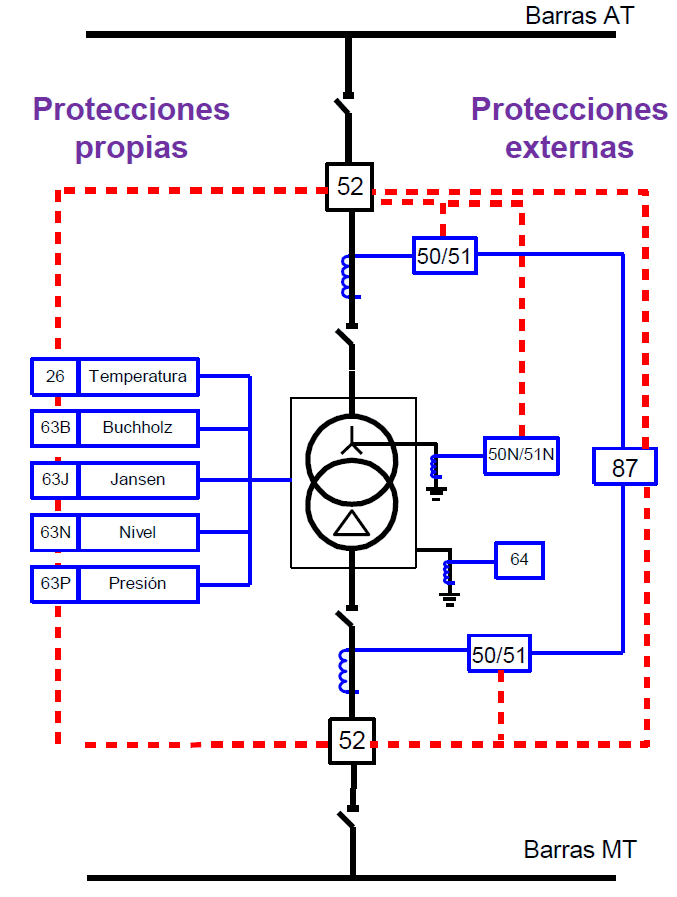
\includegraphics[width=0.4\linewidth]{Images/74}
	\label{fig:74}
\end{figure}

\subsection{Comparación entre fusibles y relés de protección}
\begin{figure}[H]
	\centering
	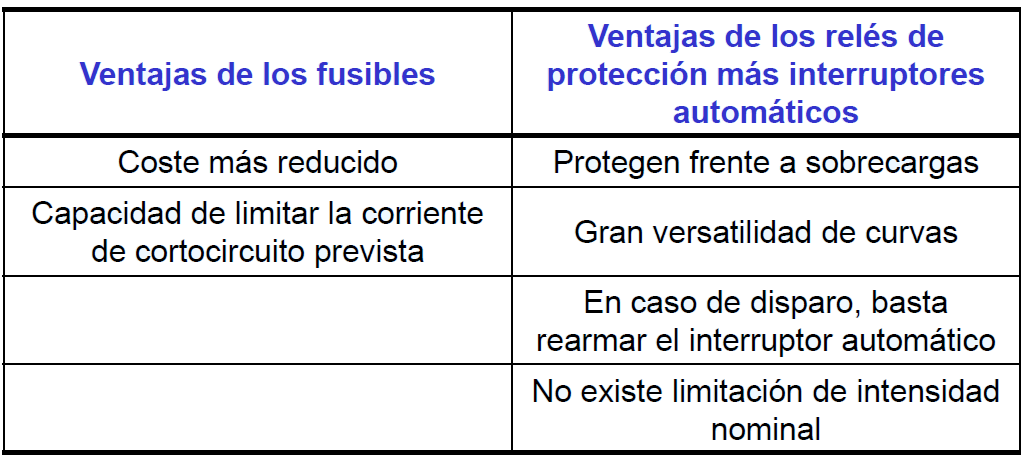
\includegraphics[width=0.5\linewidth]{Images/75}
	\label{fig:75}
\end{figure}

\section{Funcionamiento de un transformador en régimen de sobrecarga}
\begin{itemize}
	\item \textbf{Carga asignada o continua}: carga que un transformador puede suministrar de forma continua a la tensión y frecuencias asignadas y a la temperatura ambiente de diseño, sin que sobrepasen los límites de calentamiento del aceite o aislamiento y del punto más caliente del arrollamiento
	\item \textbf{Carga cíclica}: carga con variaciones cíclicas de duración habitual 24 horas
	\begin{enumerate}
		\item \textbf{Carga cíclica normal}:
		\begin{enumerate}
			\item Carga que provoca el mismo envejecimiento térmico que la carga asignada a temperatura ambiente de diseño
			\item Durante una parte del ciclo: el transformador funciona con una temperatura ambiente más elevada o con una corriente de carga superior al valor asignado
			\item Durante otra parte del ciclo: el transformador trabaja con una temperatura ambiente más baja o una carga más baja, que compensa las sobrecargas
			\item No supone un envejecimiento mayor que la carga asignada
			
		\end{enumerate}
		\item \textbf{De emergencia de larga duración}:
		\begin{enumerate}
			\item Consecuencia de la indisponibilidad prolongada de elementos de la red que no se volverán a conectar antes de que el transformador alcance una temperatura estabilizada nueva y más alta a la del régimen permanente
			\item Si persiste durante semanas o incluso meses puede suponer un considerable envejecimiento del transformador, pero no un riesgo de fallo prematuro
		\end{enumerate}
		\item \textbf{De emergencia de corta duración}:
		\begin{enumerate}
			\item Carga excepcionalmente alta, de naturaleza transitoria (típicamente menor de 30 minutos), debida a la aparición de uno o varios eventos poco probables que perturban seriamente la carga normal del sistema
			\item Supone un incremento de riesgo de fallo ya que se incrementa la temperatura del punto caliente en los conductores reduciendo temporalmente su resistencia dieléctrica.
			\item Es preferible mantener al transformador trabajando en estas condiciones que una pérdida de suministro.
			\item La duración admisible de esta carga es más corta que la constante de tiempo térmico del transformador y depende de la temperatura de funcionamiento antes del aumento de la carga
		\end{enumerate}
	\end{enumerate}
	\item En función de la clase térmica del aislamiento existen límites en la sobrecarga y en la temperatura admisible que no deben darse simultáneamente.
\end{itemize}
\section{Protección de transformadores frente a sobrecargas}
\begin{enumerate}
	\item \textbf{Protección básica:} control de la temperatura de los arrollamientos
	\begin{enumerate}
		\item La medida no puede realizarse directamente en el devanado. Se mide el aceite o el aislamiento.
		\item Transformadores en aceite: Termostato
		\begin{enumerate}
			\item Temperatura del aceite en el nivel superior de la cuba
			\item Ajuste del termostato: menor a 115$\angle$C
		\end{enumerate}
		\item Transformadores de tipo seco: Sondas de temperatura
		\begin{enumerate}
			\item Posibilidad de temperaturas muy distintas en los devanados de las distintas fases en caso de desequilibrio. Al menos: dos sensores por arrollamiento
			\item Ajuste del sensor: menor a la temperatura límite indicada en la norma
		\end{enumerate}
	\end{enumerate}
	\item \textbf{Protección complementaria:} Relé de sobreintensidad de tiempo inverso ajustando su curva de disparo a las condiciones de carga previstas del transformador
	\begin{enumerate}
		\item Regulaciones por defecto para transformadores en aceite:
		\begin{enumerate}
			\item Permitir trabajar al trafo con carga cíclica normal y de emergencia de larga duración durante tiempo indefinido (supone protección por termostato). \textbf{Protección no dispara para esta corriente}
			\item Disparo antes de media hora para carga de emergencia de corta duración
		\end{enumerate}
		\item Regulaciones para transformadores en seco:
		\begin{itemize}
			\item No disparar por debajo de un valor inferior a 1.5 la intensidad nominal
			\item Disparar siempre que se alcance 1.5 el valor de la intensidad nominal 
		\end{itemize}
	\end{enumerate}
\end{enumerate}
Trafos en aceite:
\begin{figure}[H]
	\centering
	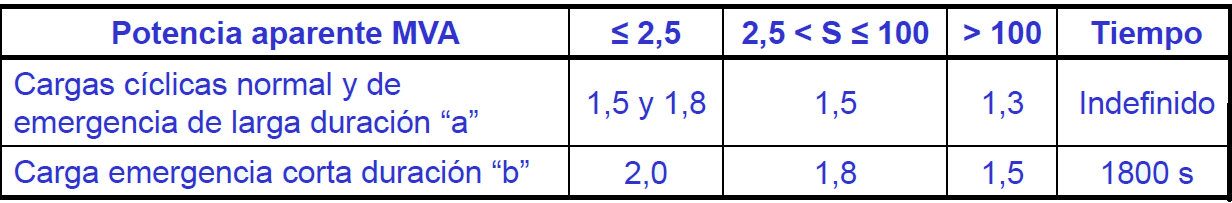
\includegraphics[width=0.7\linewidth]{Images/76}
	\label{fig:76}
\end{figure}

Trafos secos: En un determinado ciclo de carga la intensidad nominal no debe exceder de 1,5 veces la nominal.
\subsection{Protección mediante relés de imagen térmica}
\begin{enumerate}
	\item Permite seleccionar la velocidad de envejecimiento relativa admisible
	\item El relé ajusta su curva de disparo para que la temperatura del punto más caliente garantice la velocidad de envejecimiento admisible
	\item \textbf{Funcionamiento del relé de imagen térmica:} calculan la temperatura del punto más caliente del transformador mediante las siguiente medidas:
	\begin{enumerate}
		\item Corriente de carga del transformador
		\item Temperatura
	\end{enumerate}
	\item \textbf{Tipos de relés de imagen térmica:}
	\begin{enumerate}
		\item Sencillos: miden la temperatura ambiente y estiman la temperatura del aceite en la parte superior de la cuba mediante modelo
		\item Sofisticados: miden la temperatura del aceite en la parte superior de la cuba y calculan la temperatura del punto más caliente del arrollamiento mediante modelo
	\end{enumerate}
	\item La curva de actuación del relé de imagen térmica se ajusta automáticamente según se la temperatura ambiente medida
\end{enumerate}
\section{Protección de transformadores frente a cortocircuitos}
\subsection{Tipos de categorías de transformadores trifásicos según potencia}
\begin{itemize}
	\item Categoría I: 25 kVA a 2500 kVA
	\item Categoría II: 2501 kVA a 100 MVA
	\item Categoría III: mayor de 100 MVA
\end{itemize}
\subsection{Cálculo de la corriente de cortocircuito}
Se debe de realizar teniendo en cuenta la impedancia de cortocircuito del transformador más la impedancia de la red. Para los transformadores de categoría I: se puede despreciar la impedancia de la red, si:
\begin{equation}
	Z_{red}\le 5\% Z_{CC_T}
\end{equation}
\subsection{Valores mínimos reconocidos de la impedancia de cortocircuito para los transformadores de dos arrollamientos separados.}
\begin{table}[H]
	\centering
	\begin{tabular}{|c|c|}
		\hline
		\textbf{Potencia asignada (kVA)} & \textbf{Impedancia de cortocircuito mínima (\%)} \\
		\hline
		25 a 630 & 4 \% \\
		631 a 1250 & 5 \% \\
		1251 a 2500 & 6 \% \\
		2501 a 6300 & 7 \% \\
		6301 a 25000 & 8 \% \\
		25001 a 40000 & 10 \% \\
		40001 a 63000 & 11 \% \\
		63001 a 100000 & 12.5 \% \\
		Mayor que 100000 & $> 12.5 \%$ \\
		\hline
	\end{tabular}
\end{table}
\subsection{Efectos térmicos}
El transformador debe soportar la corriente de cortocircuito simétrica, calculada
de acuerdo a las indicaciones de la norma, durante 2 s, manteniendo la temperatura
media de cada arrollamiento por debajo de los valores especificados en dicha norma.
\newline

Si se desprecia la impedancia de lata tensión:
\begin{equation}
	I_{k2s}=\dfrac{cU_f}{Z_T}=\dfrac{cI_n}{\varepsilon_{cc}}
\end{equation}

Con este valor de corriente se obtiene la curva térmica (una recta en escala logarítmica):
\begin{equation}
	I_k^2\cdot t= cte =I_{k2s}^2\cdot 2s
\end{equation}

\textbf{Se ajusta la protección de tal manera que la curvar $I^2t$ quede por encima, que la sobrecarga de corta duración se despeje en 1800s y que las sobrecargas de larga duración no provoquen el disparo. Para ello, se usan las gráficas de las curvas de disparo. Además no ha de disparar en el arranque.}
\newline

\textbf{La curva de disparo instantáneo debe disparar en 0,1s a partir de la intensidad de cortocircuito. Puede disparar antes pero no después. Se debe de comprobar el poder de corte.}
\begin{figure}[H]
	\centering
	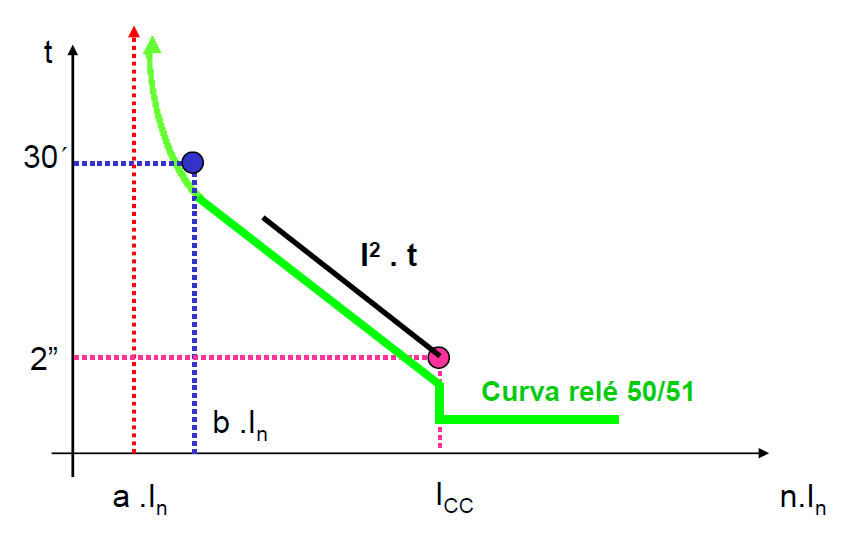
\includegraphics[width=0.7\linewidth]{Images/77}
	\label{fig:77}
\end{figure}

\subsection{Ajustes de la curva de disparo}
\begin{itemize}
	\item No debe disparar la protección del trafo de alta antes que lo haga la protección del lado de baja
	\item Para valores superiores a $I_{k2s}$ la protección del trafo debe actuar lo más rápido posible ya que corresponderá a un defecto interno o un defecto en bornes de alta tensión del transformador limitado por una impedancia de cortocircuito inferior a la del trafo y que no es visto por la protección de baja tensión
\end{itemize}
\subsection{Efectos electrodinámicos}
Se usa  el valor $\kappa$ para calcular el valor pico:
\begin{equation}
	I_p=\sqrt{2}\kappa I_k
\end{equation}
Para calcular $\kappa$:
\begin{equation}
	\kappa=1,02+0,98e^{-\dfrac{3R}{X_L}}
\end{equation}